%%%%%%%%%%%%%%%%%%%%%%%%%%%%%%%%%%%%%%%%%
% Beamer Presentation
% LaTeX Template
% Version 2.0 (March 8, 2022)
%
% This template originates from:
% https://www.LaTeXTemplates.com
%
% Author:
% Vel (vel@latextemplates.com)
%
% License:
% CC BY-NC-SA 4.0 (https://creativecommons.org/licenses/by-nc-sa/4.0/)
%
%%%%%%%%%%%%%%%%%%%%%%%%%%%%%%%%%%%%%%%%%

%----------------------------------------------------------------------------------------
%	PACKAGES AND OTHER DOCUMENT CONFIGURATIONS
%----------------------------------------------------------------------------------------

\documentclass[
	11pt, % Set the default font size, options include: 8pt, 9pt, 10pt, 11pt, 12pt, 14pt, 17pt, 20pt
	%t, % Uncomment to vertically align all slide content to the top of the slide, rather than the default centered
	%aspectratio=169, % Uncomment to set the aspect ratio to a 16:9 ratio which matches the aspect ratio of 1080p and 4K screens and projectors
]{beamer}

\graphicspath{{Images/}{./}} % Specifies where to look for included images (trailing slash required)

\usepackage{booktabs} % Allows the use of \toprule, \midrule and \bottomrule for better rules in tables

%----------------------------------------------------------------------------------------
%	SELECT LAYOUT THEME
%----------------------------------------------------------------------------------------

% Beamer comes with a number of default layout themes which change the colors and layouts of slides. Below is a list of all themes available, uncomment each in turn to see what they look like.

%\usetheme{default}
%\usetheme{AnnArbor}
%\usetheme{Antibes}
%\usetheme{Bergen}
%\usetheme{Berkeley}
%\usetheme{Berlin}
%\usetheme{Boadilla}
%\usetheme{CambridgeUS}
%\usetheme{Copenhagen}
%\usetheme{Darmstadt}
%\usetheme{Dresden}
%\usetheme{Frankfurt}
%\usetheme{Goettingen}
%\usetheme{Hannover}
%\usetheme{Ilmenau}
%\usetheme{JuanLesPins}
%\usetheme{Luebeck}
\usetheme{Madrid}
%\usetheme{Malmoe}
%\usetheme{Marburg}
%\usetheme{Montpellier}
%\usetheme{PaloAlto}
%\usetheme{Pittsburgh}
%\usetheme{Rochester}
%\usetheme{Singapore}
%\usetheme{Szeged}
%\usetheme{Warsaw}

%----------------------------------------------------------------------------------------
%	SELECT COLOR THEME
%----------------------------------------------------------------------------------------

% Beamer comes with a number of color themes that can be applied to any layout theme to change its colors. Uncomment each of these in turn to see how they change the colors of your selected layout theme.

%\usecolortheme{albatross}
%\usecolortheme{beaver}
%\usecolortheme{beetle}
%\usecolortheme{crane}
%\usecolortheme{dolphin}
%\usecolortheme{dove}
%\usecolortheme{fly}
%\usecolortheme{lily}
%\usecolortheme{monarca}
%\usecolortheme{seagull}
%\usecolortheme{seahorse}
%\usecolortheme{spruce}
%\usecolortheme{whale}
%\usecolortheme{wolverine}

%----------------------------------------------------------------------------------------
%	SELECT FONT THEME & FONTS
%----------------------------------------------------------------------------------------

% Beamer comes with several font themes to easily change the fonts used in various parts of the presentation. Review the comments beside each one to decide if you would like to use it. Note that additional options can be specified for several of these font themes, consult the beamer documentation for more information.

\usefonttheme{default} % Typeset using the default sans serif font
%\usefonttheme{serif} % Typeset using the default serif font (make sure a sans font isn't being set as the default font if you use this option!)
%\usefonttheme{structurebold} % Typeset important structure text (titles, headlines, footlines, sidebar, etc) in bold
%\usefonttheme{structureitalicserif} % Typeset important structure text (titles, headlines, footlines, sidebar, etc) in italic serif
%\usefonttheme{structuresmallcapsserif} % Typeset important structure text (titles, headlines, footlines, sidebar, etc) in small caps serif

%------------------------------------------------

%\usepackage{mathptmx} % Use the Times font for serif text
\usepackage{palatino} % Use the Palatino font for serif text
%\usepackage{helvet} % Use the Helvetica font for sans serif text
\usepackage[default]{opensans} % Use the Open Sans font for sans serif text
%\usepackage[default]{FiraSans} % Use the Fira Sans font for sans serif text
%\usepackage[default]{lato} % Use the Lato font for sans serif text

%----------------------------------------------------------------------------------------
%	SELECT INNER THEME
%----------------------------------------------------------------------------------------

% Inner themes change the styling of internal slide elements, for example: bullet points, blocks, bibliography entries, title pages, theorems, etc. Uncomment each theme in turn to see what changes it makes to your presentation.

%\useinnertheme{default}
\useinnertheme{circles}
%\useinnertheme{rectangles}
%\useinnertheme{rounded}
%\useinnertheme{inmargin}

%----------------------------------------------------------------------------------------
%	SELECT OUTER THEME
%----------------------------------------------------------------------------------------

% Outer themes change the overall layout of slides, such as: header and footer lines, sidebars and slide titles. Uncomment each theme in turn to see what changes it makes to your presentation.

%\useoutertheme{default}
%\useoutertheme{infolines}
%\useoutertheme{miniframes}
%\useoutertheme{smoothbars}
%\useoutertheme{sidebar}
%\useoutertheme{split}
%\useoutertheme{shadow}
%\useoutertheme{tree}
%\useoutertheme{smoothtree}

%\setbeamertemplate{footline} % Uncomment this line to remove the footer line in all slides
%\setbeamertemplate{footline}[page number] % Uncomment this line to replace the footer line in all slides with a simple slide count

%\setbeamertemplate{navigation symbols}{} % Uncomment this line to remove the navigation symbols from the bottom of all slides

%----------------------------------------------------------------------------------------
%	PRESENTATION INFORMATION
%----------------------------------------------------------------------------------------

\title[Short Title]{ENGR151 Recitation Class 2} % The short title in the optional parameter appears at the bottom of every slide, the full title in the main parameter is only on the title page

\subtitle{week 4} % Presentation subtitle, remove this command if a subtitle isn't required

\author[James Cook \and Roald Amundsen]{Wu JiaXi} % Presenter name(s), the optional parameter can contain a shortened version to appear on the bottom of every slide, while the main parameter will appear on the title slide

\institute[UC]{UM-SJTU joint institute \\ \smallskip \textit{nina$\_$nhk@sjtu.edu.cn}} % Your institution, the optional parameter can be used for the institution shorthand and will appear on the bottom of every slide after author names, while the required parameter is used on the title slide and can include your email address or additional information on separate lines

\date[\today]{Computer $\&$ Programming, MatLab-scripting \\ \today} % Presentation date or conference/meeting name, the optional parameter can contain a shortened version to appear on the bottom of every slide, while the required parameter value is output to the title slide

%----------------------------------------------------------------------------------------

\begin{document}

%----------------------------------------------------------------------------------------
%	TITLE SLIDE
%----------------------------------------------------------------------------------------

\begin{frame}
	\titlepage % Output the title slide, automatically created using the text entered in the PRESENTATION INFORMATION block above
\end{frame}

%----------------------------------------------------------------------------------------
%	TABLE OF CONTENTS SLIDE
%----------------------------------------------------------------------------------------

% The table of contents outputs the sections and subsections that appear in your presentation, specified with the standard \section and \subsection commands. You may either display all sections and subsections on one slide with \tableofcontents, or display each section at a time on subsequent slides with \tableofcontents[pausesections]. The latter is useful if you want to step through each section and mention what you will discuss.

\begin{frame}
	\frametitle{Presentation Overview} % Slide title, remove this command for no title
	
	\tableofcontents % Output the table of contents (all sections on one slide)
	%\tableofcontents[pausesections] % Output the table of contents (break sections up across separate slides)
\end{frame}

%----------------------------------------------------------------------------------------
%	PRESENTATION BODY SLIDES
%----------------------------------------------------------------------------------------

\section{Playbook Review} % Sections are added in order to organize your presentation into discrete blocks, all sections and subsections are automatically output to the table of contents as an overview of the talk but NOT output in the presentation as separate slides

%------------------------------------------------
\begin{frame}
	\textbf{Disclaimer:}\\
    The answers provided here are not guranteed to be correct. Please
    use them as a references only and verify with reliable source.

    \smallskip

    \textbf{Note:}\\
     only go through some questions that we think they are necessary.
	
\end{frame}

%------------------------------------------------
\subsection{C2}
%------------------------------------------------


\begin{frame}
	\frametitle{C2 Playbook Review}
	\textbf{2.1.1 What is the terminal mode of MATLAB?}
	\bigskip % Vertical whitespace
	
    \quad In terminal mode, MATLAB operates entirely through the \textbf{command line interface (CLI)} \\
	\quad This mode allows you to execute commands and scripts directly from the terminal or command line.
    \begin{figure}
        \centering
        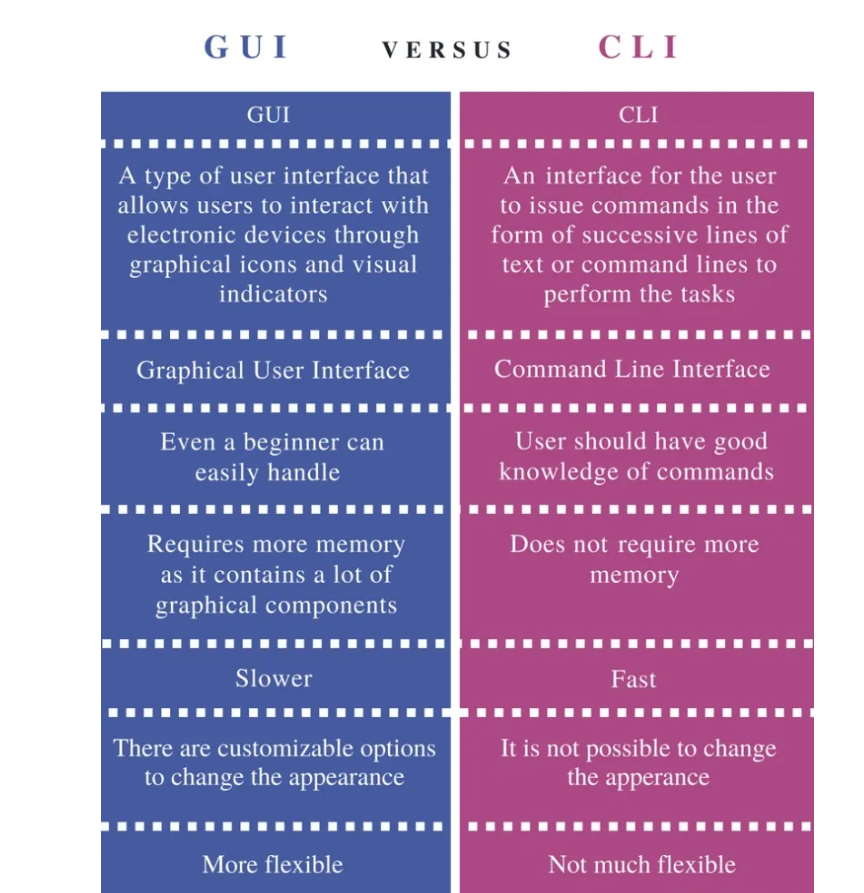
\includegraphics[width=0.4\textwidth]{diff_gui_and_cli.png}
        \caption{The difference between GUI \& CLI.}
    \end{figure}
\end{frame}

%------------------------------------------------

\begin{frame}
	\frametitle{C2 Playbook Review}
	\textbf{2.1.4What is the difference between clc and clearvars?}
	\begin{itemize}
        \item \texttt{clc}: Clears the \textbf{command window}.
        It erases all text and output currently visible in the command window, but it \textbf{does not affect the workspace variables or any of the data in memory}.
        \item \texttt{clearvars}: Clears \textbf{variables from the workspace}.It removes the specified variables from memory, freeing up the workspace.
    \end{itemize}
	\smallskip
    \textbf{Usecases}
	\begin{itemize}
        \item \texttt{clc}: to clean up the command window when it becomes cluttered with output.
        \item \texttt{clearvars}: to free up memory or reset the workspace by removing variables you no longer need.
    \end{itemize}

    \smallskip

    \textbf{Note}: use \texttt{help} command for quick search of function.
\end{frame}

%------------------------------------------------

\begin{frame}
	\frametitle{C2 Playbook Review}
	\textbf{2.1.6 What is the difference between an array and a matrix? }
    \begin{figure}
        \centering
        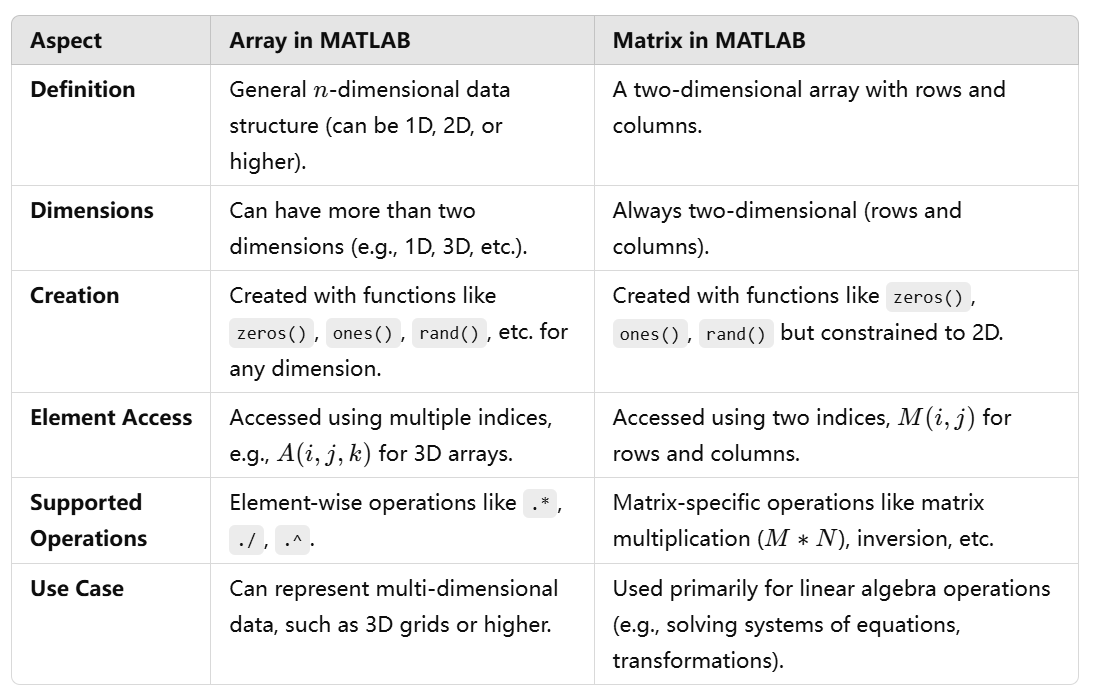
\includegraphics[width=0.85\textwidth]{array_matrix.png}
    \end{figure}

    \textbf{Note}: More here \href{https://www.mathworks.com/help/matlab/matlab_prog/array-vs-matrix-operations.html}{[Link toward documentation]}
\end{frame}

%------------------------------------------------

\begin{frame}
	\frametitle{C2 Playbook Review}
	\textbf{2.1.6 What is the conjugate of a real number? }
    
    \quad The conjugate of a real number is the same as the real number itself, because real numbers have no imaginary part. For complex numbers, the conjugate is obtained by changing the sign of the imaginary part.

    \texttt{Use conj{var} to find conjugation of a number}

    \bigskip

    \textbf{2.1.6 What should you test to see the difference between A' and A.'? }

    \begin{enumerate}
        \item randomly create a simple matrix 
        \item test it out in Matlab
        \item observe the output
    \end{enumerate}

    e.g\\
    \texttt{A = [1+2i, 2-3i; 3+4i, 4-5i];}
    \end{frame}

%------------------------------------------------

%------------------------------------------------

\begin{frame}
	\frametitle{C2 Playbook Review}
    \texttt{$A = [1+2i, 2-3i; 3+4i, 4-5i];$}

    \bigskip

    \begin{itemize}
        \item \texttt{$A'$}:
        \\ 
        \[
        A' = \begin{bmatrix}
        1 - 2i & 3 - 4i \\
        2 + 3i & 4 + 5i
        \end{bmatrix}
        \]
        \\ transpose and conjugate matrix
        \item \texttt{$A.'$}:
        \\
        \[
        A.' = \begin{bmatrix}
        1 + 2i & 3 + 4i \\
        2 - 3i & 4 - 5i
        \end{bmatrix}
        \]
        \\ only transpose matrix
    \end{itemize}
    \end{frame}


 %------------------------------------------------

\begin{frame}
	\frametitle{C2 Playbook Review}
	\textbf{2.1.6 Benefit of using help rather than the documentation}
    \begin{itemize}
        \item quick and efficient
        \item text-base and light-weight
        \item shows you the most relevant, concise details about a specific function
    \end{itemize}
    
    More comparision:

    \begin{figure}
        \centering
        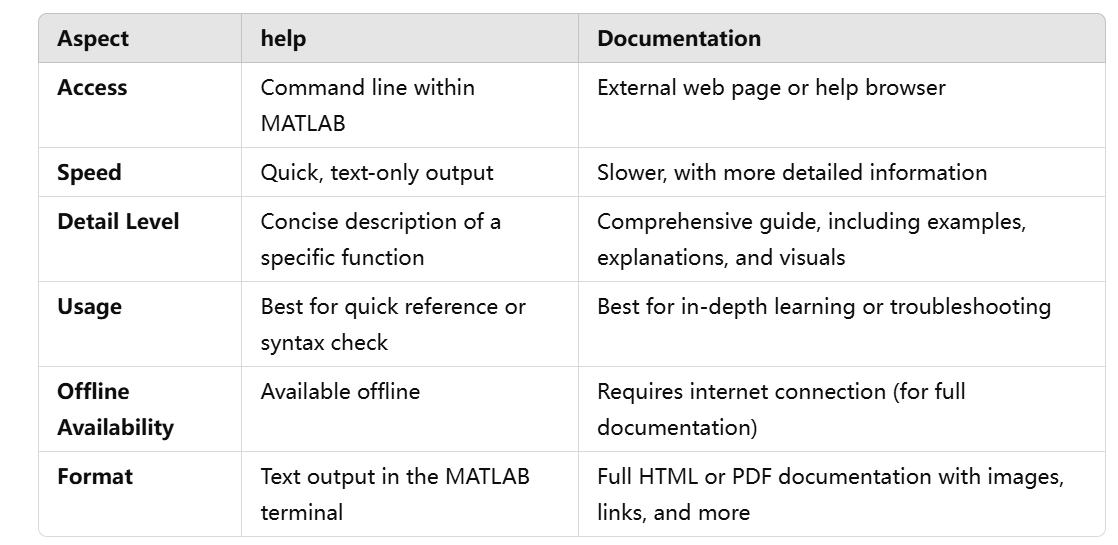
\includegraphics[width=0.85\textwidth]{doc_help.png}
    \end{figure}
    \end{frame}

%------------------------------------------------
\begin{frame}
    \frametitle{C2 Playbook Review}
    \textbf{2.1.8 In MATLAB when scanning a matrix, in what order are elements read?}

    In MATLAB, elements are read \textbf{column-wise by default}.

    \begin{itemize}
        \item About row and column indices: $A(i,j)$, where $i$ is the row index and $j$ is the column index.
        \item It iterates over columns first, then rows.
    \end{itemize}

    For example, 
    \begin{center}
        \[
        A = \begin{bmatrix}
        1 & 2 & 3 \\
        2 & 5 & 6\\
        \end{bmatrix}
        \]
    \end{center}
    It is read in the order: $A(1,1)=1$, $A(2,1)=4$, $A(1,2)=2$, $A(2,2)=5$, $A(1,3)=3$, $A(2,3)=6$.
\end{frame}

%------------------------------------------------

\begin{frame}
    \frametitle{C2 Playbook Review}
    \textbf{2.2.2 What is the difference between $A \& B$ and $A \&\& B$?}
    
    \textbf{For $A \& B$:}
    \begin{itemize}
        \item Checks each condition.
        \item $A$ and $B$ can work with arrays or matrices but must be of the same size.
        \item Slower due to element-wise checks.
    \end{itemize}
    
    \textbf{For $A \&\& B$:}
    \begin{itemize}
        \item If the first expression is false, the second expression is not evaluated (short-circuit evaluation).
        \item $A$ and $B$ must be scalar conditions (evaluate to single true/false values).
        \item Faster and more efficient.
    \end{itemize}
    \textbf{2.2.3 Explain when to prefer switch over if:}
    \begin{itemize}
        \item Use \textbf{switch} when dealing with multiple specific cases related to a single variable.
        \item Use \textbf{if} when conditions are varied, involve comparisons, or require logical operations.
    \end{itemize}
    
\end{frame}
%------------------------------------------------

\begin{frame}
    \frametitle{C2 Playbook Review}
    discuss the code in C2.\\(you should be able to answer the following questions)
    \begin{figure}
        \centering
        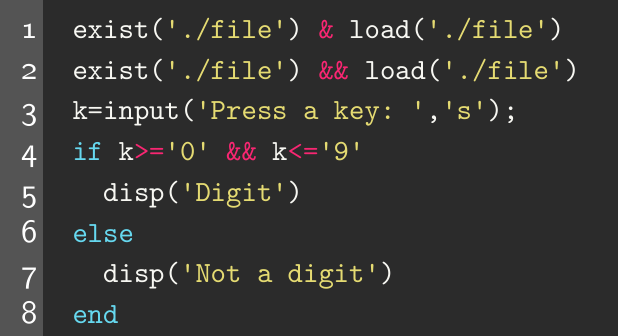
\includegraphics[width=0.5\textwidth]{c2_15.png}
    \end{figure}
    
    \begin{itemize}
        \item \textbf{The difference between lines 1 and 2.}
        \item \textbf{Why is k compared to '0' between quotes and not 0'?}
        \item \textbf{Why is the first script returning an error when more than one key is pressed?}
    \end{itemize}

\end{frame}

%------------------------------------------------

\begin{frame}
    \frametitle{C2 Playbook Review}
    \textbf{2.3.2 If str2num() is replaced by str2double() is the script still working?}
    \begin{figure}
        \centering
        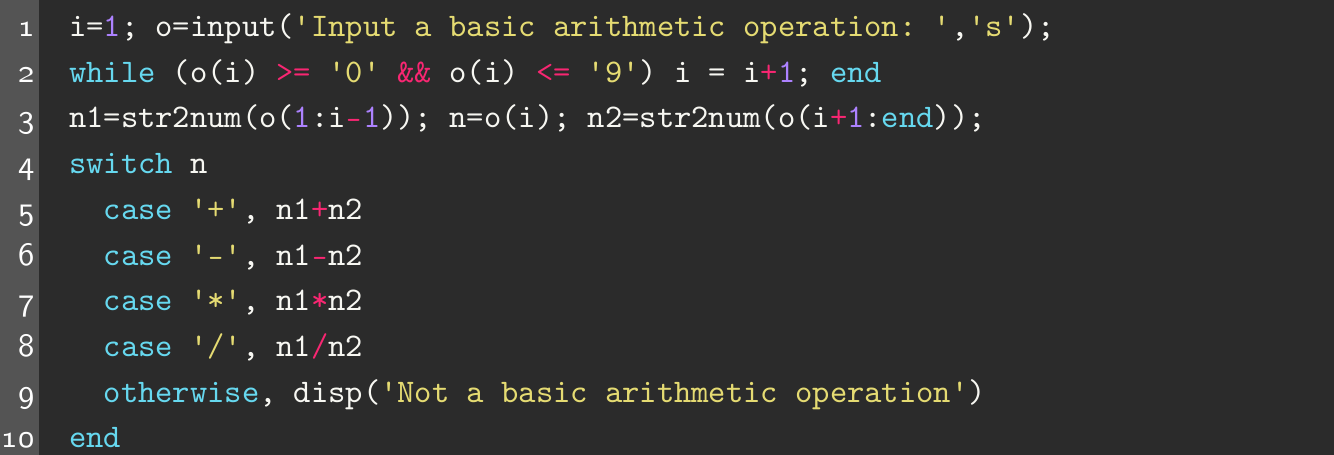
\includegraphics[width=0.6\textwidth]{c2_18.png}
    \end{figure}


\end{frame}


%------------------------------------------------



\begin{frame}
    \frametitle{C2 Playbook Review}
    \textbf{2.3.6 How useful are the continue and break commands?}
    \begin{itemize}
        \item \texttt{continue}
        \begin{itemize}
            \item \textbf{Purpose}: It skips the remaining code in the current iteration of a loop and proceeds to the next iteration.
            \item \textbf{Use Case}: helpful when skipping certain iterations based on a condition without terminating the entire loop. 
        \end{itemize}
        \item \texttt{break}
        \begin{itemize}
            \item \textbf{Purpose}: It terminates the loop entirely and transfers control to the statement following the loop.
            \item \textbf{Use Case}: Useful when you want to exit a loop prematurely based on a condition.
        \end{itemize}
       \end{itemize}
    
    \textbf{2.3.6 Why is it important not to abuse those commands?}
    
    \begin{itemize}
        \item lower code readiblity as the logic become more complicated
        \item Easily causing logic error in which functions are not working as intended
        \item use condition statement for better control
    \end{itemize}

\end{frame}


%------------------------------------------------

\begin{frame}
    \frametitle{C2 Playbook Review}
    \textbf{2.3.4 What does it mean for the code to be indented?}\\
    It refers to the practice of adding spaces or tabs at the beginning of lines to visually represent the structure and hierarchy of the code.Which then helps increases code readability.
    Having good practice of indented code is important.
    
    \bigskip

    \textbf{2.3.10 What is a logical mask?}
    A logical mask in MATLAB is an array of logical values (true or false) that can be used to index or filter elements in another array. It allows you to selectively access or manipulate parts of an array based on certain conditions. 
    \\ for example
    \\\texttt{A = [1, 2, 3, 4, 5];}
    \\\texttt{mask = A > 3; \% This will result in [false, false, false, true, true]}

\end{frame}

%------------------------------------------------

\begin{frame}
    \frametitle{C2 Playbook Review}

    \begin{figure}
        \centering
        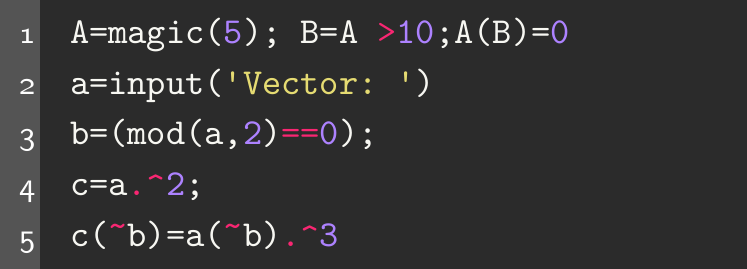
\includegraphics[width=0.6\textwidth]{c2_26.png}
    \end{figure}

    \textbf{2.3.10 What is the mod() function doing?}

    \textbf{2.3.10 Given a $5\times5$ matrix A, use the mod() function to determine the row of A(14).}

   
    
\end{frame}

%---

\subsection{C3}
\begin{frame}
	\frametitle{C3 Playbook review}
    \textbf{3.1.1 Clearly explain the difference between script and function}
    \begin{figure}
        \centering
        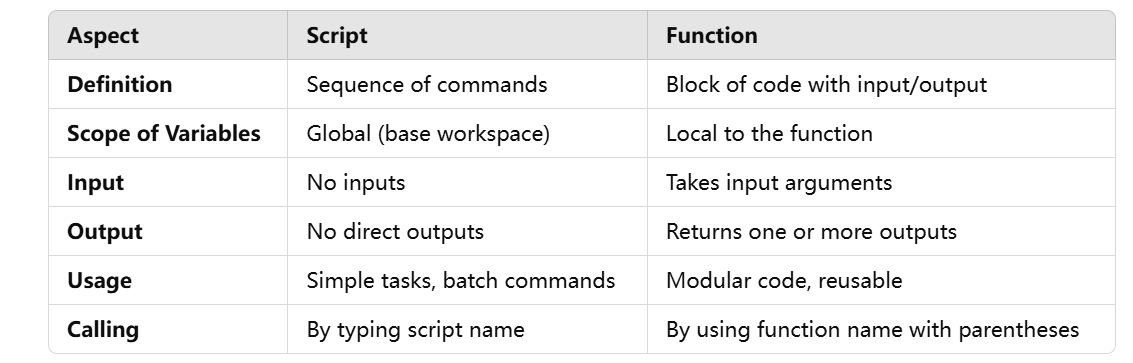
\includegraphics[width= 0.8\textwidth]{script_function.png}
    \end{figure}
\end{frame}


%------------------------------------------------

\begin{frame}
	\frametitle{C3 Playbook review}
    \textbf{3.1.3 Clearly explain what is a "sub-function"?}

    In MatLab, sub-functions are written after the main function in the same file, and they can only be called by the main function or other sub-functions within the file. 

    \textbf{3.1.3Why are sub-functions very useful, and should be use as much as possible?}
    
    \begin{itemize}
        \item As sub-functions \textbf{are not visible or accessible from outside the file}, making them useful for organizing code that is meant to be used internally.
        \item It allows breaking down complex tasks into smaller, manageable pieces. 
        \item It can be reused multiple times within the same file, reducing code duplication. 
        \item Easy debugging.
    \end{itemize}
\end{frame}
%------------------------------------------------
\begin{frame}
	\frametitle{C3 Playbook review}
    \textbf{3.1.3 How to catch more than one output?}

    In MatLab, we can catch more than one output by using brackets,namely \textbf{[]}.
    
    \bigskip

    for example,

    \texttt{function [sumVal, prodVal] = addAndMultiply(x, y)}

    \texttt{ \quad sumVal = x + y;}

    \texttt{ \quad prodVal = x * y;}

    \texttt{end}
\end{frame}
%------------------------------------------------

\begin{frame}
	\frametitle{C3 Playbook review}
    \textbf{3.2.1 Explain in simple terms what is recursion.}
   
    Recursion is when a function calls itself to solve a problem.
    \begin{enumerate}
        \item The function keeps calling itself.
        \item Each call gets closer to a base case, which is a simple scenario where the function doesn't call itself anymore.
        \item Once the base case is reached, the function returns a result, and all the previous calls can finish.
    \end{enumerate}
    \begin{itemize}
        \item Base case: The stopping point where the function doesn't call itself.
        \item Recursive step: The part where the function calls itself with a simpler problem.
    \end{itemize}
\end{frame}
%------------------------------------------------
%------------------------------------------------

\begin{frame}
	\frametitle{C3 Playbook review}
    \textbf{3.2.2 Explain in simple terms the basic difference between iteration and recursion.}
    \begin{figure}
        \centering
        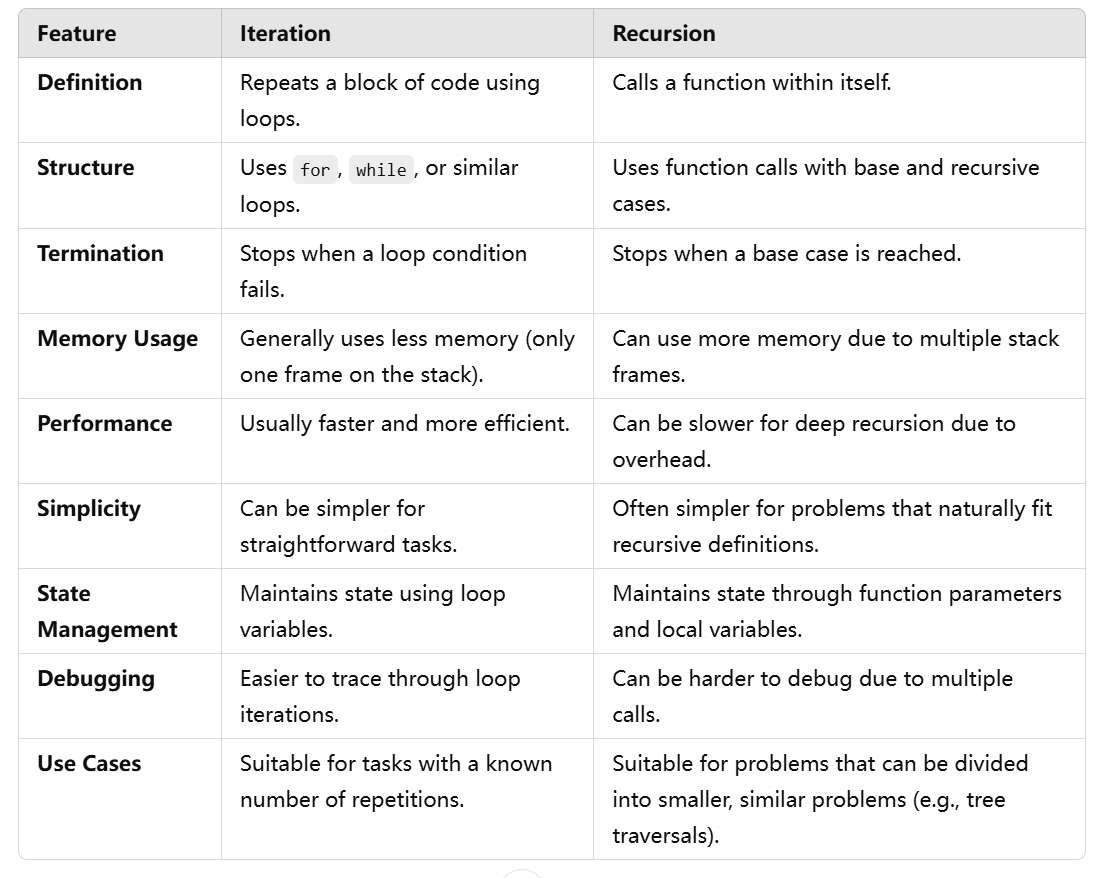
\includegraphics[width=0.9\textwidth]{iter_recur.png}
    \end{figure}
\end{frame}
%------------------------------------------------
%------------------------------------------------

\begin{frame}
	\frametitle{C3 Playbook review}
    \textbf{3.2.8 Explain why recursion can cause some memory issues?}
    \begin{itemize}
        \item \textbf{Stack Overflow}: Too many recursive calls can exhaust the stack memory, leading to a crash.
        \item \textbf{Memory Inefficiency}: Recursion can lead to inefficient use of memory, especially in cases of redundant calculations, because each recursive call maintains its own state on the stack.
    \end{itemize}
\end{frame}
%------------------------------------------------
%------------------------------------------------

\begin{frame}
	\frametitle{C3 Playbook review}
    \textbf{3.2.8 Implement the generation of Fibonacci numbers using (i) iteration and (ii) recursion.}
    \begin{itemize}
        \item iteration \\
        \begin{enumerate}
            \item Input a non-negative integer n.
            \item if n == 0, return 0 / If n == 1, return 1./ iterates f = f0 + f1
            \item sum the result and output the n-th Fibonacci number.
        \end{enumerate}
        \item recursion\\
        \begin{enumerate}
            \item Input a non-negative integer n.
            \item if n == 0, return 0 / If n == 1,return 1/ return fibonacci(n-1) + fibonacci(n-2)
            \item output result
        \end{enumerate}
    \end{itemize}
\end{frame}
%------------------------------------------------
%------------------------------------------------

\begin{frame}
	\frametitle{C3 Playbook review}

    \textbf{iteration}

\texttt{function f = fibonacci\_iter(n)} \\
\texttt{  \quad  if n == 0} \\
\texttt{    \quad  \quad     f = 0;} \\
\texttt{    \quad else if n == 1} \\
\texttt{    \quad  \quad     f = 1;} \\
\texttt{    \quad else} \\
\texttt{     \quad  \quad    f0 = 0;} \\
\texttt{ \quad  \quad f1 = 1;} \\
\texttt{    \quad  \quad     for i = 2:n} \\
\texttt{      \quad  \quad  \quad       f = f0 + f1;} \\
\texttt{      \quad  \quad  \quad       f0 = f1;} \\
\texttt{  \quad  \quad  \quad       f1 = f;} \\
\texttt{      \quad  \quad   end} \\
\texttt{   \quad  end} \\
\texttt{end} \\
\end{frame}

%------------------------------------------------

\begin{frame}
	\frametitle{C3 Playbook review}

    \textbf{recursion}

    \texttt{function f = fibonacci\_rec(n)} \\
    \texttt{  \quad  if n == 0} \\
    \texttt{  \quad  \quad       f = 0;} \\
    \texttt{  \quad   elseif n == 1} \\
    \texttt{   \quad  \quad      f = 1;} \\
    \texttt{  \quad   else} \\
    \texttt{  \quad  \quad       f = fibonacci\_rec(n-1) + fibonacci\_rec(n-2);} \\
    \texttt{  \quad   end} \\
    \texttt{end}
\end{frame}
\begin{frame}
%------------------------------------------------
	\frametitle{C3 Playbook review}
    \textbf{3.2.8 What is a "seed"?}
    A seed is an initial value used to start a random number generator, which is like the starting point for a sequence. 
    By using a seed, you can control the sequence of "random" numbers that are produced.
    \textbf{3.2.8 What is happening if the same seed is used to generated random numbers?}
    If you use the same seed each time, the random number generator will produce the same sequence of numbers every time. 
    This can be useful when you want to reproduce results (for debugging or testing), but it also means the numbers aren't truly random. 

\end{frame}

%------------------------------------------------

\begin{frame}
    \frametitle{C3 Playbook Review}
    
    \textbf{3.3.3 What does it mean to "print in a string"?} \\
    "Printing in a string" refers to inserting values into a string using special formatting symbols. Instead of just printing plain text, you can include variables or values inside a string. This is done using format specifiers like \texttt{\%d} (for integers) or \texttt{\%f} (for floats).
    
    \textbf{3.2.8 How to know what flags (e.g., \texttt{\%d}, \texttt{\%g}) or special characters (e.g., \texttt{\\n}, \texttt{\\t}) should be used?}
    - Read the documentation for \texttt{sprintf} or \texttt{fprintf}.
    
    Format specifiers are used to format different data types:
    \begin{itemize}
        \item \texttt{\%d}: For integers (decimal).
        \item \texttt{\%f}: For floating-point numbers (decimals).
        \item \texttt{\%s}: For string.
        \item \texttt{\%c}: For char.
        \item \texttt{\%g}: For the most compact representation of a floating-point number (either \texttt{\%f} or scientific notation, \texttt{\%e}).
    \end{itemize}

    Special characters are used to control how the output looks:
    \begin{itemize}
        \item \texttt{\\n}: Newline (moves to the next line).
        \item \texttt{\\t}: Tab (inserts a horizontal tab space).
    \end{itemize}

\end{frame}



%------------------------------------------------

\begin{frame}
	\frametitle{C3 Playbook review}
    \textbf{3.3.5 What are the dangers of not closing a file?}
    \begin{itemize}
        \item The system keeps the file open in memory, which uses resources unnecessarily and can slow down the program.
        \item  The file might remain locked, preventing other programs or users from accessing or modifying it.
        \item   Data might not be written or saved properly, leading to file corruption.
    \end{itemize}
    \textbf{3.3.5 Why should files be opened as for "as little time as possible"?}
    \begin{itemize}
        \item Opening a file uses system resources (memory and file handles), and the sooner you close it, the more resources are freed for other tasks.
        \item The longer a file is open, the greater the chance of issues like crashes, file corruption, or conflicts with other programs.
        \item Closing a file ensures that all data is written and saved properly, reducing the risk of data loss or corruption.
    \end{itemize}
\end{frame}

%------------------------------------------------

\section{Worksheet Review}

\subsection{W3}

\begin{frame}
	\textbf{Note:} For some questions, we won't directly provide the entire source code.
    Instead, we will provide ideas, a piece of code or pseudo-code to help guide you through worksheet questions.
\end{frame}


%------------------------------------------------

\begin{frame}
	\frametitle{Ex 1}
	
	\textbf{Ensure you can answer all the questions in C3 sildes}

    \bigskip
    \bigskip

    \quad go through the slide yourself and \textbf{make sure you are familiar with all concepts mentioned.}
\end{frame}


%------------------------------------------------

\begin{frame}
	\frametitle{Ex2}
	
	\textbf{Read Matlab documentation for the following functions:}
	
	\smallskip % Vertical whitespace
	\begin{block}{functions}
        save, load, $(s|f)$ printf, rand, fopen,fclose,randperm
    \end{block}
	\bigskip

    Note: \\ use \textbf{$"help  + function\_name"$} to search for documentation effectively.
	
	\end{frame}

%------------------------------------------------

\begin{frame}
	\frametitle{Ex2}
	
	\textbf{save}
	
    \begin{itemize}
        \item Purpose: Saves workspace variables to a file.
        \item Syntax:
            \begin{itemize}
                \item \texttt{save(filename)}: Saves all variables in the workspace to the file filename.
                \item \texttt{save(filename, variables)}: Saves the specified variables to the file filename.
                \item \texttt{save(filename, variables, '-append')}: Appends variables to an existing file.
            \end{itemize}
    \end{itemize}
    \smallskip
    \textbf{load}
	
    \begin{itemize}
        \item Purpose: Loads variables from a file into the workspace.
        \item Syntax:
            \begin{itemize}
                \item \texttt{load(filename)}: Loads all variables from the file filename.
                \item \texttt{load(filename, variables)}: Loads only the specified variables from the file.
            \end{itemize}
    \end{itemize}
	
	
	\end{frame}
%------------------------------------------------

\begin{frame}
    \frametitle{Ex2}

	\textbf{(s$|$f)printf}
	
    \begin{itemize}
        \item Purpose: Formats data into a string (sprintf) or writes formatted data to a file or command window (fprintf).
        \item Syntax:
            \begin{itemize}
                \item \texttt{sprintf(formatSpec, A1, ..., An)}: Formats the data according to formatSpec and returns it as a string.
                \item \texttt{fprintf(formatSpec, A1, ..., An)}: Writes the formatted data to the screen or a file.
            \end{itemize}
    \end{itemize}
    \smallskip
    \textbf{rand} 
	
    \begin{itemize}
        \item Purpose: Returns a scalar from a uniform distribution in the interval (0,1).
        \item Syntax:
            \begin{itemize}
                \item \texttt{rand}: Returns a scalar from a uniform distribution in the interval (0,1).
                \item \texttt{rand(n)}: Returns an n-by-n matrix of random numbers.
                \item \texttt{rand(m,n)}: Returns an m-by-n matrix of random numbers.
            \end{itemize}
    \end{itemize}
\end{frame}

%------------------------------------------------

\begin{frame}
    \frametitle{Ex2}

    \textbf{fopen}
    
    \begin{itemize}
        \item Purpose: Opens a file for reading, writing, or appending.
        \item Syntax:
            \begin{itemize}
                \item \texttt{file\_id = fopen(filename, mode)}: Opens the file and returns a file identifier (file\_id).
                \item Modes:
                    \begin{itemize}
                        \item \texttt{r}: Read (file must exist).
                        \item \texttt{w}: Write (creates a new file or overwrites an existing one).
                        \item \texttt{a}: Append (writes to the end of the file).
                    \end{itemize}
            \end{itemize}
    \end{itemize}
    \smallskip
    \textbf{fclose}
    
    \begin{itemize}
        \item Purpose: Closes an open file.
        \item Syntax:
            \begin{itemize}
                \item \texttt{fclose(file\_id)}: Closes the file associated with the file identifier \texttt{file\_id}.
                \item \texttt{fclose('all')}: Closes all open files.
            \end{itemize}
        \item \textbf{Remember to close the file every time you open one!}
    \end{itemize}
\end{frame}

%------------------------------------------------

\begin{frame}
    \frametitle{Ex2}

    \textbf{randperm}
    
    \begin{itemize}
        \item Purpose: Returns a row vector containing a random permutation of integers.
        \item Syntax:
            \begin{itemize}
                \item \texttt{randperm(n)}: Returns a random permutation of the integers from 1 to n.
                \item \texttt{randperm(n, k)}: Returns k unique integers selected randomly from 1 to n.
            \end{itemize}
    \end{itemize}
\end{frame}
%------------------------------------------------

\begin{frame}
	\frametitle{Ex3}

	\textbf{Solve the problem (3.22|3.103) using an alternative algorithm and different Matlab functions.}
    
\end{frame}
%------------------------------------------------
\begin{frame}
	\frametitle{Ex3}

	\textbf{Objective:} Solve the problem using different algorithms and MATLAB functions.
    \begin{itemize}
        \item Explore alternative string splitting functions.
        \item Investigate other functions to randomly select lines from a file.
        \item Propose a different algorithm to solve the problem.
    \end{itemize}
\end{frame}
%------------------------------------------------

\begin{frame}
	\frametitle{Ex3}

	\textbf{1. Alternative functions for splitting strings:}
    \begin{itemize}
        \item \texttt{strsplit(string)}
        \item \texttt{regexp(string, pattern, 'split')}
    \end{itemize}
    
    \textbf{2. Functions for picking random lines:}
    \begin{itemize}
        \item \texttt{randi([1, file\_total\_length])} 
    \end{itemize}
    
    \textbf{3. Alternative algorithm:}
    \begin{itemize}
        \item Read the file, identify the target line, and extract the required string.
        (Note: This might be redundant but could work in specific cases.)
    \end{itemize}
\end{frame}

%------------------------------------------------

\begin{frame}
	\frametitle{Ex4}

	\textbf{Dicuss the following recursion}

    A child couldn't sleep, so her mother told her a story about a little frog, who couldn't sleep, so the frog's mother told her a story about a little bear, who couldn't sleep, so the bear's mother told her a story about a little weasel who fell asleep. …and the little bear fell asleep; …and the little frog fell asleep; …and the child fell asleep.
    
    \bigskip
    For an automated information service a telephone company needs the digits of phone numbers to be read digit by digit. Design an algorithm allowing to rewrite an sequence of digits into words, with a space between each word, but no space at the beginning and at the end.

    \textbf{what are the base cases?}
    \\ \textbf{Try to Implement the second algorithm}

\end{frame}

%------------------------------------------------

\begin{frame}
   \begin{figure}
        \centering
        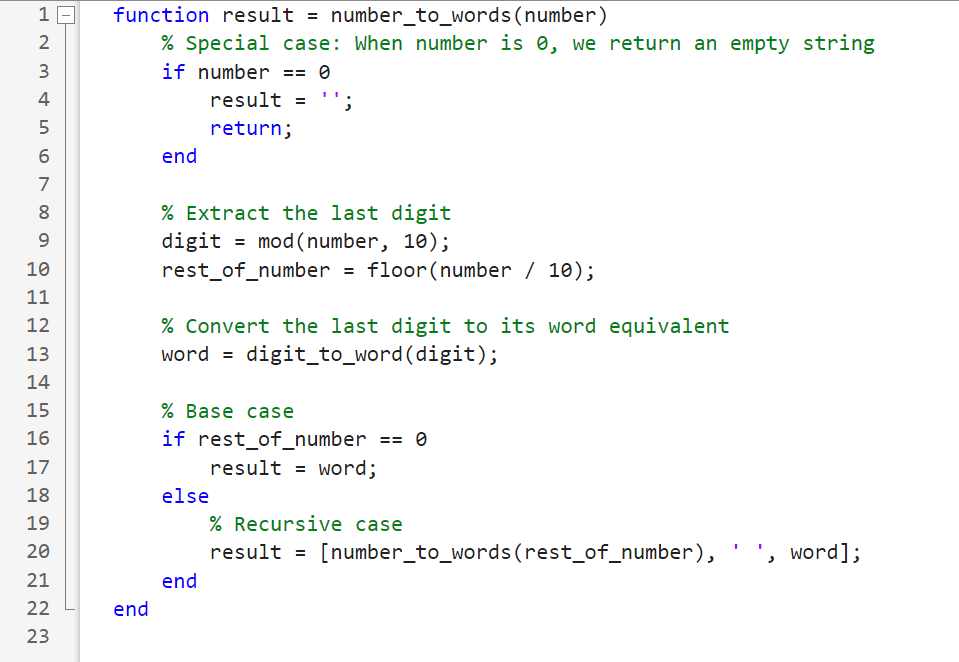
\includegraphics[width=0.9\textwidth]{ex4.png}
   \end{figure}
\end{frame}

%------------------------------------------------

\begin{frame}
    \frametitle{Ex5}
    For any integer \(n\), we define its successor \(S(n) = n + 1\). 
    For any \(x, y \in \mathbb{N}\), let \(f\) be the function defined by:
    \[
    f(x, 0) = 0
    \]
    \[
    f(x, S(y)) = g(f(x, y), x),
    \]
    where \(g\) is such that
    \[
    g(x, 0) = x
    \]
    \[
    g(x, S(y)) = S(g(x, y)).
    \]
    \textbf{Manually calculate f (0,0), f (1,0), f (1,1), f (2,1), f (2,2), and f (2,3).}
    \\
    \textbf{Using words explain what you guess the function f is doing.}
    
    \quad Function \texttt{f} is recursively multiplying \texttt{x} and \texttt{y}. 
    With the behavior of the helper function \texttt{g}, it builds up the result by adding \texttt{x} to the previous result \texttt{y} times.
   
    \textbf{What is the base case and recursive case here?}
\end{frame}

%------------------------------------------------

\begin{frame}
    \frametitle{Ex5}

    \textbf{Implement it and test it on larger inputs.}
    \begin{block}{sample function}
        \texttt{function result = f(x, y)}
        \\\quad \texttt{if y == 0}
        \\\quad  \quad \texttt{result = 0; \% Base case}
        \\\quad   \texttt{else}
        \\\quad  \quad \texttt{result = g(f(x, y-1), x); \% Recursive case}
        \\\quad   \texttt{end}
    \\\texttt{end}
\\
    \texttt{ function result = g(x, y)}
    \\\quad \texttt{if y == 0}
    \\\quad  \quad \texttt{ result = x; \% Base case}
    \\\quad   \texttt{else}
    \\\quad  \quad \texttt{ result = g(x, y-1) + 1; \% Recursive case}
    \\\quad   \texttt{end}
    \\\texttt{end}
   
    \end{block}

\end{frame}


%------------------------------------------------

\begin{frame}
	\frametitle{Ex6}

	\textbf{ Write a MATLAB program composed of a single command to sum up all integers from 0 to n.}
    
    \bigskip
    
    \bigskip

    \textbf{Write a simple iterative MATLAB program to sum up all integers from 0 to n.}
    
    \bigskip

\end{frame}

%------------------------------------------------

\begin{frame}
	\frametitle{Ex6}

	\textbf{ a single command to sum up all integers from 0 to n.}

    \texttt{sum = n * (n + 1) / 2;}
    
    \textbf{a simple iterative MATLAB program to sum up.}
    \begin{itemize}
        \item sum function \\ \texttt{sum = sum(0:n);}
        \item while \\ \texttt{while i <= n} \\ \quad \texttt{sum = sum + i; }\\\quad \texttt{ i = i + 1;}\\\texttt{end}
        \item for \\ \texttt{for i = 0:n} \\\quad \texttt{sum = sum + i; }\\\texttt{end}
    \end{itemize}

\end{frame}

%------------------------------------------------

\begin{frame}
	\frametitle{Ex6}
   \textbf{Now write a simple recursive MATLAB program to sum up all integers from 0 to n.}
   \begin{itemize}
    \item What is the base case?
    \\
    \item What actions occur at each level of the recursion?
    \\
    \item Draw a simple diagram showing the recursion progress.
   \end{itemize}

\end{frame}

%------------------------------------------------

\begin{frame}
	\frametitle{Ex6}
   \begin{itemize}
    \item \textbf{What is the base case?}
    \\ For different algorithm, there will be different base cases.
    In the diagram I provided, the base cases will be \textbf{n=0;}
    \item  \textbf{What actions occur at each level of the recursion?}
    \item \textbf{ Draw a simple diagram showing the recursion progress.}
    \begin{figure}
        \centering
        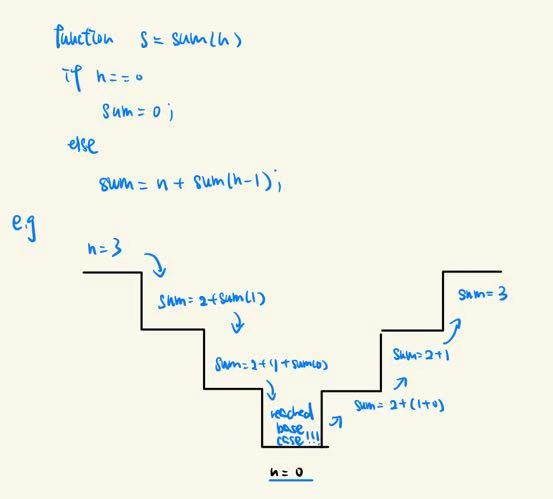
\includegraphics[width=0.4\textwidth]{ex6_recursion_diagram.jpg}
    \end{figure}
   \end{itemize}

\end{frame}

%------------------------------------------------

\begin{frame}
	\frametitle{Ex6}
   ideas given, try to fill in the blanks!
   \\

   \begin{block}{\quad \quad recsum.m}
    \texttt{function s = \_\_\_\_\_(n)} \\
    \texttt{\ \ \ \ if n == \_\_\_\_\_} \\
    \texttt{\ \ \ \ \ \ \ \ s = \_\_\_\_\_;} \\
    \texttt{\ \ \ \ else} \\
    \texttt{\ \ \ \ \ \ \ \ s = \_\_\_\_\_ + \_\_\_\_\_;} \\
    \texttt{\ \ \ \ end}
    
   \end{block}
\end{frame}

%------------------------------------------------
\begin{frame}
	\frametitle{Ex6}
    \textbf{reference code}

    \bigskip

    \texttt{function s= recsum(n) \% pay attention to the file name as this file only contain this function!}
    \\\quad \texttt{if n == 0}
    \\\quad  \quad \texttt{s = 0;}
    \\\quad   \texttt{else}
    \\\quad  \quad \texttt{s = n + recsum(n - 1); }
    \\\quad   \texttt{end}
\\\texttt{end}

\end{frame}

%------------------------------------------------
\section{Referencing}

\begin{frame} 
	\frametitle{References}
	
	\begin{itemize}
        \item Manuel.
    \end{itemize}
\end{frame}

%----------------------------------------------------------------------------------------
%	CLOSING SLIDE
%----------------------------------------------------------------------------------------

\begin{frame}[plain] % The optional argument 'plain' hides the headline and footline
	\begin{center}
		{\Huge The End}
		
		\bigskip\bigskip % Vertical whitespace
		
		{\LARGE Questions? Comments?}
	\end{center}
\end{frame}

%----------------------------------------------------------------------------------------

\end{document} 